\chapter{Experimental Setups}
\label{ch:exptsetup}

In all experiments in this thesis, a flow circuit was used to contain the blood and provide control over parameters like oxygenation.
This circuit is similar to what is used in cardio-pulmonary bypass surgery, where a patient's blood is pumped and oxygenated by a heart lung machine.
Over the course of this research, the experimental setup was improved, leading to two main versions - the original stopped flow setup, and the continuous flow setup.

\section{Stopped flow experimental setup}
\label{sec:exptsetup-stopflow}

\subsection{Flow circuit and pump}
\begin{figure}
\centering
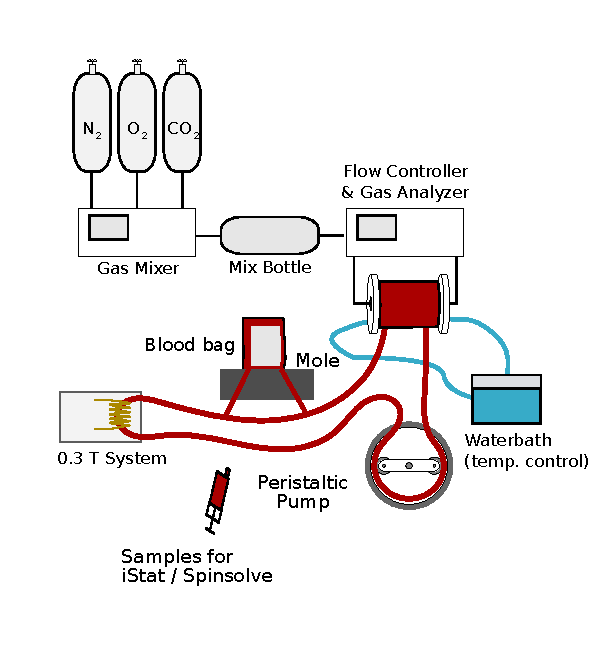
\includegraphics[width=0.8\textwidth]{figures/exptsetup/BloodMixingSetup.pdf}
\caption{Schematic of the Stopped flow setup}
\label{fig:exptsetup-stopflowschematic}
\end{figure}

A schematic of the flow stopped setup is shown in \autoref{fig:exptsetup-stopflowschematic}.
The main components are the roller pump and the oxygenation membrane, with the blood collection bag acting as a reservoir.
These are all joined by 1/4'' medical grade PVC tubing.
The total volume of this circuit was typically \SI{60}{\milli\litre}, with the blood bag containing 450 ml TODO check logbook.

The roller pump is used to generate flow around the circuit, by rotating the pump head to drive 2 rollers that squeeze the walls of the tube and force the blood along.
The pump is also designed for use in CPB surgery, and is a Stockert SIII, with a flow rate controllable from \SIrange{0.01}{6}{L/m} when used with the 1/4'' tube. TODOcheck?.
These versions of the flow circuit included a bypass section controlled by clamping the tubes so that the blood flow could be directed to around the reservoir, allowing for faster changes in the oxygenation due to a lower effective volume.
One important setting on the pump is the occlusion, which controls how much the tubing is squeezed as the pump head rotates.
Having the occlusion set too loosely causes the pump to become ineffective, as the blood can flow backwards through the pump, while setting it too tightly was found to cause damage to the red blood cells as they travel through the pump.
One problem with the model of pump used in these experiments does not have any sort of readout of the occlusion setting, so this had to be set at the correct value by following a testing procedure each time the occlusion was changed.

\subsection{Oxygenator and Gas Mixer}
A hollow-fibre membrane oxygenator was used to control the oxygenation of the blood in the circuit.
This was a Medtronic Affinity Pixie oxygenator, designed for use in paediatric CPB procedures.
It allows for gas exchange and temperature control of the blood flowing through, with the oxygenation controlled by the mix of gases going into the oxygenator.
This paediatric model was chosen to minimize the required priming volume, and it still provided more than enough capacity to oxygenate the blood at the flow rates used.
The temperature of the blood was regulated by flowing water from a temperature controlled waterbath through the oxygenator, which has a separate path built into it for this purpose.
The water bath temperature was set to \SI{35}{\degreeCelsius}, although this corresponded with a blood temperature at the outlet of \SI{33}{\degreeCelsius} at maximum flow rates (with lower temperatures at lower flow rates.)

The gas mix was set using a Dansensor MapMix 3 gas mixer, which allowed control of the different proportions of \Ntwo, \Otwo, and \COtwo flowing through the oxygenator.
The Oxygen fraction was typically varied from 0\% up to 21\%, the value of atmospheric air.
Nitrogen was used as a non-Oxygen containing gas, and between 2.5-5\% \COtwo was also added to ensure the pH of the blood sample remained stable over the course of the experiment (as these are linked by the bicarbonate buffer system in blood).
Gases for all experiments were used as supplied from BOC and were instrument grade or higher.
The output of the gas mixer flowed into a pressurised buffer tank before flowing into a Dansensor MapCheck Provectus gas analyser, which allowed us to check the fraction of the three gases which flowed into the oxygenation membrane.
This gas analyser also provided some flow regulation, although this was supplemented with an adjustable flow valve.
Typically, the gas flow rate was set to only \SIrange[per-mode=symbol]{1}{2}{\liter\per\minute} to avoid creating bubbles in the oxygenator.

\subsection{Blood collection}
Samples of whole blood were collected by venipuncture from healthy volunteers (taking place at Otago medical school).
This procedure was approved by the central health and disability ethics committee, and all volunteers provided written, informed consent.
Approximately \SI{450}{ml} of blood was collected into a blood bag containing \SI{66.5}{\milli\litre} CPD anticoagulant/preservative solution (Haemonetics Leukotrap WB system).
CPD solution is rated for storage of red blood cells for up to at least 3 weeks of storage\cite{Hessupdatesolutionsred2006}.
Blood samples were held at room temperature following collection, before undergoing leukoreduction filtering to remove white blood cells.
As it has been shown that the presence of white blood cells can adversely affect the condition of red blood cells in storage\cite{Hessupdatesolutionsred2006}.
Samples were then moved to a refrigerator and stored at \SI{4}{\degreeCelsius} until required for experiments (up to 30 TODO check! days for stopped flow experiments, up to 10 days for continuous flow experiments)

\subsection{NMR setup}
For these experiments, 3 different permanent magnet systems were used to obtain data at 3 different field strengths.
TODO pics of magnets!!

The first system was a 12 MHz (\SI{0.3}{T}) Halbach magnet array, with \SI{9}{cm} diameter bore and approximately \SI{20}{\centi\metre} long.
This magnet was repurposed from a previous experiment in the lab, and specifications are not available for it.
When combined with the home built coil and holder system described in \autoref{sec:exptsetup-coil}, the FID linewidth produced by the magnet was \SI{12}{\kilo\hertz}, which is relatively broad.

Because it uses permanent magnets, it requires a stable temperature in order to have a stable field.
This was set up using a temperature controlled water bath, which pumped wat at a constant \SI{30}{\celsius} through tubes wrapped around the magnet.
On top of this, the magnet was wrapped in a layer of foam, and a layer of mylar sheeting to insulate it from the room.
To decrease the effect of electrical noise on the measurements, the magnet assembly was also surrounded by a thin coppper mesh blanket.

The second magnet system used was the NMR MOLE, previously developed by Manz et al\cite{ManzmobileonesidedNMR2006}.
The NMR MOLE operates at a field of \SI{0.1}{T} and is a single sided device, which produces a `sweet spot' in the region above the magnet.
The sweet spot is where the combination of magnetic field and RF produced by the coil on the surface are able to create resonance, which defines where signal comes from.
In this case, the sweet spot was a pair of regions marking out a \SI{3}{cm} circle over the RF coil (TODO see figure? honours project).
While earlier experiments attempted to position the tube containing blood over the sweet spot, in later experiments, it was decided that it was simpler and more reliable to place the blood bag on the top of the MOLE.
As with the Halbach array, the MOLE is also sensitive to temperature, so an electronic temperature controller and wire heater were used to keep it stable at \SI{29}{\celsius}.

The design of the magnet array in the MOLE creates strong magnetic field gradients across the sweet spot.
This creates a wide range of resonance frequencies, and means that it was not possible to measure an FID from the system.
It was also found that this limited the possible range of CPMG echo times, as echo times longer than \SI{1}{ms} were caused excessive signal attenuation.
This limited experiments with this system to short echo times.

The third magnet system used was a Magritek Spinsolve, which is another permanent magnet based NMR system operating at \SI{1}{T}.
The Spinsolve is designed for chemical spectroscopy, so has a very homogeneous field, and can produce a linewidth of less than \SI{0.1}{Hz}.
It also uses standard 5 mm NMR sample tubes, so it could not be used inline in the flow circuit like the other two systems.
Because of this, experiments on the Spinsolve required withdrawing a small amount of blood and transferring it into an NMR tube.
This meant that that there were typically delays between removing the blood from the circuit and taking measurements on it, which may cause changes in the state of the blood.

Both the Halbach and MOLE systems were controlled on computers running Magritek Prospa, and used Magritek Kea 2 spectrometers to run the NMR experiments.
The Spinsolve was also controlled from a computer with a newer version of Prospa.
CPMG experiments were run using the default CPMG macros included in Prospa, with batch scripts set up to automate taking measurements at multiple echo times.

\section{Continuous flow setup}
\label{sec:exptsetup-contflow}

To be able to get better data on how \Ttwo is affected by \SOtwo at different fields, we decided to move to a continuous flow method, where the \SOtwo was slowly ramped from low to high oxygenation, while the \Ttwo was constantly measured.
This required a number of changes to the stopped flow setup, including the use of the baby-MRI magnet, and the development of a system for continuours \SOtwo tracking.


\begin{itemize}
\item Flow Circuit changes
\item different magnet
\item sO2 measurement - optical sensor, calibration
\item Flow stability
\end{itemize}

\subsection{Flow Circuit Changes}

\subsection{Coil Assemblies and Electronics}
\label{sec:exptsetup-coil}
A new coil holder, coil assembly and tuning and matching circuit was designed to fit into the baby-MRI system and also used in the Halbach magnet array experiments in  \autoref{ch:stoppedflow}.
It was designed with exchangeable coils and tuning and matching capacitors so that the probe could be used at multiple fields / frequencies.
It consists of a probe (outer piece), which holds the coil assembly and the tuning and matching circuit inside the bore of the magnet (which had the same diameter in the two magnets).

The coils are \SI{2}{cm} long, and have a diameter of \SI{1}{cm}, so that the 1/4'' tube can be passed through the coil,
Different numbers of turns were used for the three different coils, to be able to use the coils at different frequencies (More turns causes more inductance, and a lower resonant frequency.)
In the initial design of the coil assembly, the coil was constructed from \SI{0.67}{mm} Copper wire wrapped around a rolled up acetate cylinder.
A second version of the coil assemblies used 3D printed forms made from ABS plastic (to decrease unwanted signal), with the same wire and number of turns.

TODO:picture of the coils
TODO:picture of the T\&M circuit

The tuning and matching circuit was also designed and manufactured for this probe.
It allows for the capacitors to be exchanged, using small PCBs with different capacitors attached.
While high frequencies
The different capacitors allowed the probe to be tuned and matched at frequencies ranging from \SIrange{2}{60}{\mega\hertz}.
As the probe is located inside the magnet, the capacitors are all of a non-magnetic type (AVX Hi-Q or Cornell Dubilier CDE MCM series) and are rated for high voltage (\textgreater\SI{500}{V}.)
The tuning and matching circuit also contains variable capacitors which are used for fine tuning the match frequency.

S\textsubscript{11} simulations were run in Qucs Spice to find the best values of C\textsubscript{T} and C\textsubscript{M} at a range of frequencies.
